% =============================================================================
% FILE NAME : 01_fundamentals.tex
% DEPARTMENT: University of Tuebingen
% AUTOR     : Tom Schammo
% =============================================================================
% CONTENT   : Include for chapter "Fundamentals"
% =============================================================================

\section{RISC-V}

RISC-V \cite{riscv} is an open standard Instruction Set Architecture (ISA)
originally developed to support computer architecture research and education.
However, the authors now aim for RISC-V to also be used in industry implementations \cite[Cha 1]{riscv_spec}.

\subsection{ISA}

A computer program consists of several instructions.
These instructions are 'commands' that a computer understands and can react to by performing certain tasks in response.
A compiler, in case of compiled languages like C, C++, Rust, or Go, transforms code written by a human into instructions.
In case of interpreted languages like Python, Java, or JavaScript, the source code is converted into these instructions
(also sometimes referred to as 'machine code') by an interpreter or Just-In-Time (JIT) compiler during the programs' execution.
Sometimes that code is first transformed into bytecode which serves as an intermediate representation of the source code
that can be optimized.
Java, for example, is first compiled into bytecode that can be distributed and executed by the Java Virtual Machine (JVM),
whereas the python source code is often interpreted immediately line by line.
\\
An instruction set is, the set of instructions that a particular computer, or more specifically,
its Central Processing Unit (CPU) can understand.
Which instructions are available depends on the hardware of a particular system.
Instruction Set Architectures (ISA) abstractly describe the architecture of a computer.
From supported data types to available registers, to how main memory is managed by the hardware, to
which instructions a microprocessor can execute \cite{isa}.
This architecture can then be implemented by a CPU.
ISAs are often classified according to their complexity.
They either belong to the set of 'complex instruction set computers' (CISC), like x86,
or 'reduced instruction set computers' (RISC) such as ARM \cite{arm_architecture} or RISC-V \cite{riscv_spec}.

\subsection{RISC-V vs. ARM}

ARM \cite{arm} is developed by a company that sells licenses to other companies developing CPUs based on the ARM architecture,
while RISC-V \cite{riscv} is an open standard ISA provided royalty-free by 'RISC-V International', a non-profit organization.
ARM generally has a much higher market share than RISC-V due to it being used in just about every mobile device (phones, tablets, smartwatches)
these days, as well as many IoT devices and even laptops such as the new Apple MacBook containing the M1 system-on-a-chip (SOC).
However, NVIDIA announced its acquisition of ARM in 2020 \cite{arm_sale}, which was met with disapproval by some.
This led to speculation that some companies might turn to RISC-V as an alternative in the future \cite{arm_sale_speculation}.
However, the acquisition was called off in 2022 \cite{arm_sale_called_off}.\\\\
The advantage of RISC-V lies in the open nature of the standard that allows anyone to use it without paying royalties, while still
having the option to build upon the open standard.
So companies can still have their own (open or proprietary) solutions and implementations \cite{riscv_about} without having to pay for
the usage of RISC-V.

\section{Embedded AI}

As Artificial Intelligence (AI) becomes more modern and pervasive, it is only logical that it has found its way into embedded devices.
Especially with the rising trend of IoT devices and smart homes, embedded AI has found its way into the hands of consumers,
from voice assistants like Amazon's Alexa \cite{alexa} to autonomous robots like iRobot's Roomba \cite{roomba} or even self-driving cars like Tesla's Autopilot \cite{autopilot}.
However, the size and power requirements of those devices severely limit their capabilities, which is why the development of specialized hardware to improve performance
and power usage becomes a necessity.\\\\
In my thesis I'm working with the UltraTrail TC-ResNet AI Accelerator \cite{ultratrail}.
An AI Accelerator is a type of hardware accelerator specialized for artificial intelligence (AI) and machine learning (ML) applications, such as neural networks (NN).
A hardware accelerator is a set of hardware that specializes in carrying out a specific set of tasks well while sacrificing generality.
It is created to solve one type of problem faster and/or more efficiently than a generic CPU could with the trade-off that it may not be able to do other things at all.
Examples include, but are not limited to, GPUs, sound cards, cryptographic accelerators, or, in this case, AI accelerators.\\\\


\section{Rust}

The software written for this thesis, that is running on the PULPissimo \cite{pulpissimo} has been implemented using the Rust programming language \cite{rustlang}.
Rust is a relatively new general-purpose programming language that can be used to write high-performance code, comparable
to C or C++, while providing memory safety without the use of a garbage collector.
It is used for a wide variety of applications including web servers, operating systems, cryptography, and embedded devices.

\subsection{Why Rust?}

While C is the industry standard for writing software for embedded systems, along with C++ being fairly popular as well, Rust has a couple of
advantages over those languages.\\\\
The biggest downside of C is likely the lack of memory safety, which can not only cause software to be less reliable but
can also make a system vulnerable to different attacks, such as buffer overflows, reading uninitialized variables, or use-after-free, which can compromise cybersecurity \cite{memory_safety}.\\
C++ fixes some of those issues due to the availability of smart pointers, but those are fairly 'modern' C++ features, and are thus only available if compilers support more recent
versions of C++ (with C++ 11 starting to introduce many new important concepts \cite{cpp11}).
There is also no guarantee that those features have been used in any given program.
The opposite is actually more likely due to the incorporation of older software (library code written using older C++ versions),
compilers not supporting new versions (especially likely with small vendors that don't have the resources to continuously update compilers for their platform),
or developers not keeping up to date with new language features and therefore not being aware of or able to use them.\\\\
Rust on the other hand can (mostly) give compile time guarantees on the software's safety and reliability.

\begin{minipage}{\textwidth}
\subsection{Memory safety and performance}

\subsubsection{Garbage collection}

Most programming languages that try to achieve memory safety use a garbage collector for that purpose \cite{java_garbage_collector}.
A garbage collector first identifies pieces of memory that are no longer used, illustrated in Figure~\ref{fig:gc_mark}.
Then the marked pieces of memory are periodically deleted. Figure~\ref{fig:gc_delete} describes how that same chunk of memory would look after marked sections are deleted.
Finally, after the deletion, the garbage collector will 'compact' the memory to avoid memory fragmentation and improve the speed of future allocations as shown in Figure~\ref{fig:gc_compact}.
\end{minipage}

\begin{figure}[htb]
    \centering
    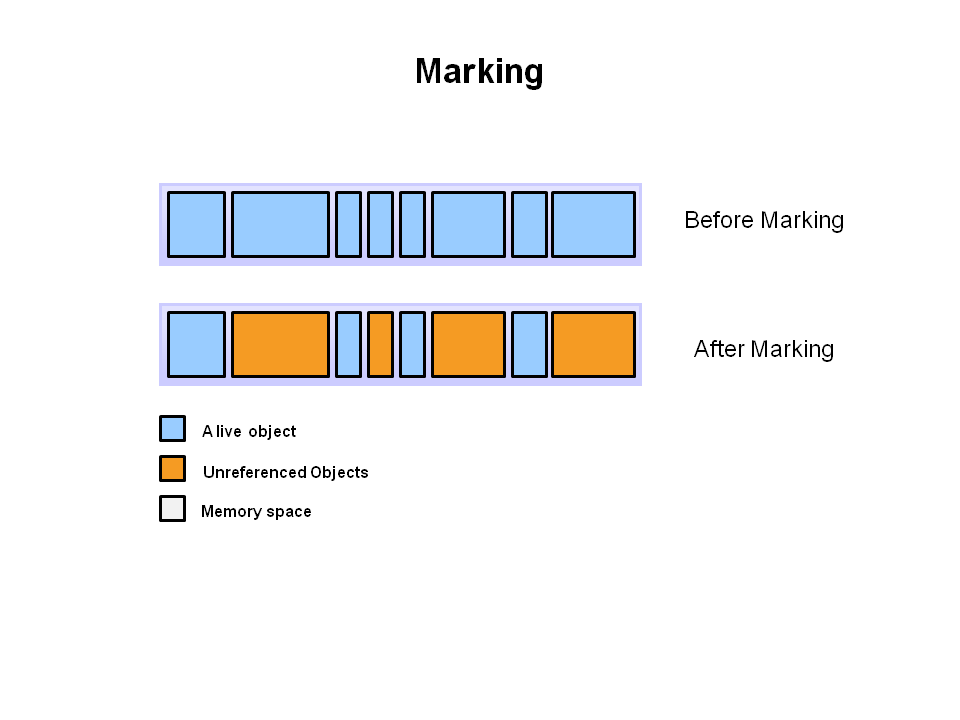
\includegraphics[width=0.9\textwidth]{figures/fundamentals_garbage_collector_marking.PNG}
    \caption[Illustration: Garbage Collector marking memory for deletion \cite{java_garbage_collector}]{Garbage Collector marking memory for deletion}
    \label{fig:gc_mark}
\end{figure}

\begin{figure}[htb]
    \centering
    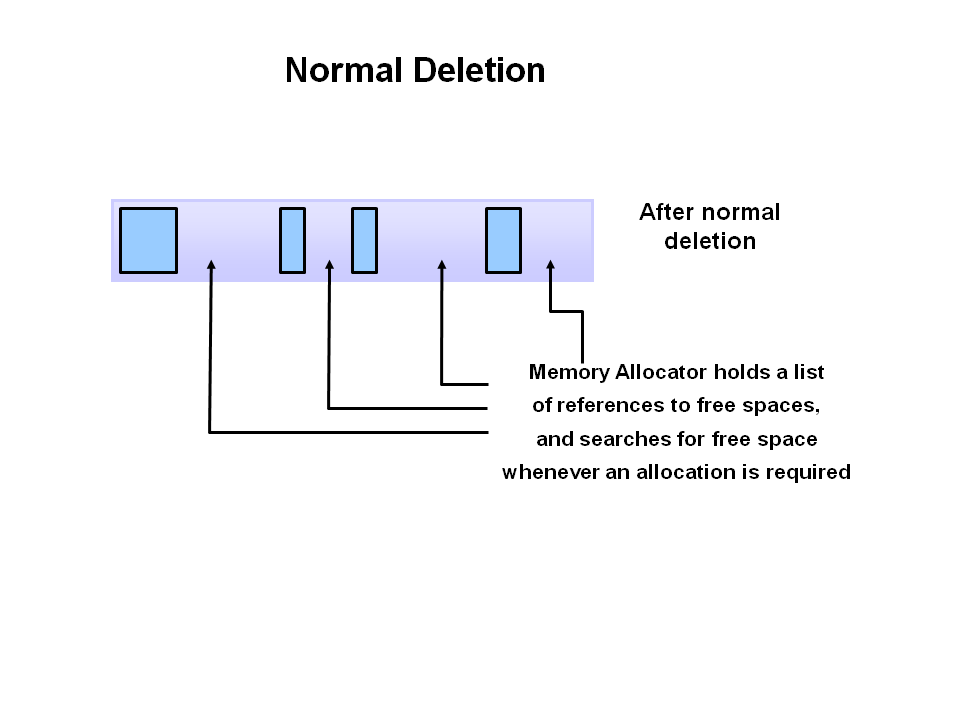
\includegraphics[width=0.9\textwidth]{figures/fundamentals_garbage_collector_deletion.PNG}
    \caption[Illustration: Garbage Collector deleting marked memory \cite{java_garbage_collector}]{Memory layout after deletion of unused pieces of memory}
    \label{fig:gc_delete}
\end{figure}

\begin{figure}[H]
    \centering
    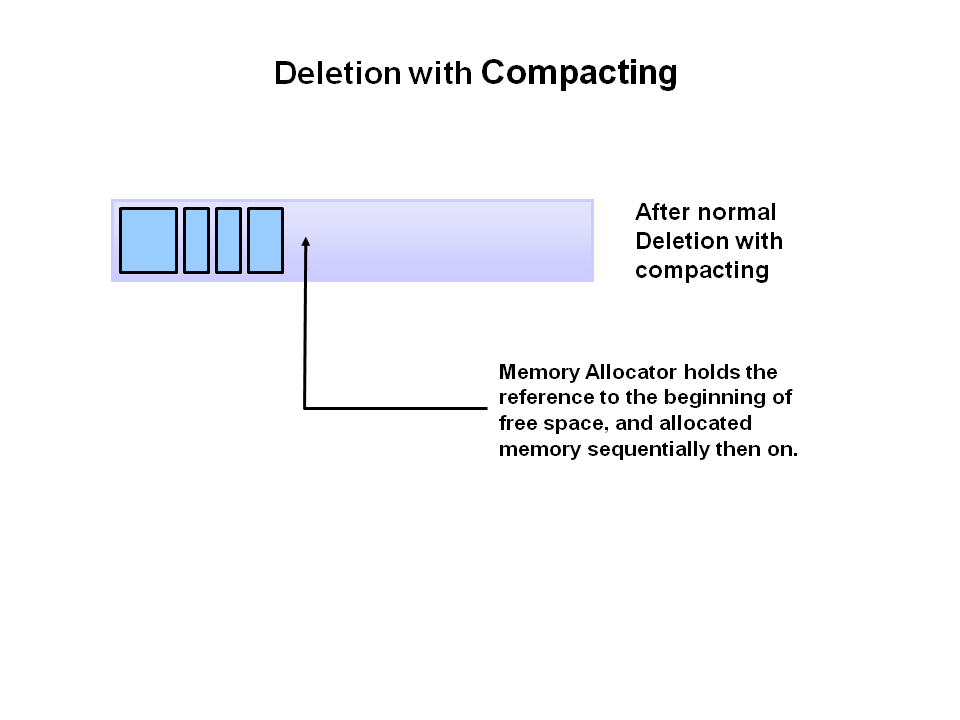
\includegraphics[width=0.9\textwidth]{figures/fundamentals_garbage_collector_compacting.PNG}
    \caption[Illustration: Garbage Collector compacting memory \cite{java_garbage_collector}]{Memory layout after compacting}
    \label{fig:gc_compact}
\end{figure}

Garbage collectors however have a few drawbacks; like unpredictable latency (the running program has to be stopped while the garbage collector is running) and a hit in performance.
The runtime of the programming language that contains the garbage collector also needs to be installed on the target system and run alongside the program
causing additional resource usage, which can be problematic in a resource-scarce environment like small embedded devices.
Therefore, garbage-collected languages are rarely used in embedded systems programming.
Rust uses a different, and unique approach to guarantee memory safety without suffering from any of the aforementioned drawbacks.

\subsubsection{Ownership in Rust}

Rust uses an 'ownership' model \cite{rust_ownership} to make memory safety guarantees at compile time and without the need for a garbage collector,
which is good for safety, and does not negatively impact performance or latency.
This model consists of 3 simple rules:
\begin{enumerate}
    \item Each value has an owner
    \item Each value can only have one owner at a time
    \item When the owner goes out of scope, the value will be dropped
\end{enumerate}

These 'owners' are generally variables. \ref{code:owner} presents a simple example of a 'value' ('\lstinline{5}') and its
'owner' ('\lstinline{owner}').\\

\begin{minipage}{\textwidth}
\begin{lstlisting}[style=colorEX,language=Rust,caption={Simple example of a value and it's owner},label={code:owner}]
let owner = 5;
\end{lstlisting}
\end{minipage}

It doesn't matter that another 'owner' might have the same value. In the code depicted in \ref{code:two_owners}
'\lstinline{owner}' and '\lstinline{owner2}' have the same value, but they are different variables, just like in any
other programming language, and have nothing to do with each other. They are different 'owners'.\\

\begin{minipage}{\textwidth}
\begin{lstlisting}[style=colorEX,language=Rust,caption={Simple example of two owners},label={code:two_owners}]
let owner = 5;
let owner2 = 5;
\end{lstlisting}
\end{minipage}


If one variable is assigned to another, one of two things happens; if the value is saved on the stack like in
example \ref{code:copy} the value is simply copied to the second variable, and now '\lstinline{owner}' and '\lstinline{owner2}'
hold the same value, but other than that have nothing to do with each other. They are different 'owners'.\\

\begin{minipage}{\textwidth}
\begin{lstlisting}[style=colorEX,language=Rust,caption={Simple example of a copy},label={code:copy}]
let owner = 5;
let owner2 = owner;
\end{lstlisting}
\end{minipage}

\begin{minipage}{\textwidth}
\begin{lstlisting}[style=colorEX,language=Rust,caption={Simple example of a move},label={code:move}]
let owner = String::from("value");
let owner2 = owner;
\end{lstlisting}
\end{minipage}

If the value is stored on the heap like in example \ref{code:move}, the value is not copied, because that could
be potentially very expensive\footnote{The more technical reason why variables for certain types cannot be copied
is that they do not implement the 'Copy' trait. This trait is only implemented for 'small' types like integers,
characters, and so on. A 'String' could theoretically be very large, while integers are limited to a few bytes at most.
However, one could implement this trait for a given type, and then it would be copied.
But this rarely makes sense for 'larger' values, because then copying is computationally expensive.
So usually the desired behavior is that those values are moved.}.
So only the pointer (memory address), the size of the data, and the capacity of the memory block are copied.
But now '\lstinline{value}' has two owners, which violates rule 2.
This rule is important because due to rule 3:
\begin{enumerate}
    \item If both variables go out of scope at the same time, the memory would be freed twice.
    \item If only one goes out of scope, the other holds the address of invalid (freed) memory.
\end{enumerate}
To avoid those things '\lstinline{value}' is considered to be 'moved' to its new owner, the variable '\lstinline{owner2}'.
The original owner ('\lstinline{owner}') is no longer valid.\\
This works similarly for functions, and these 3 rules allow the compiler to check for any mistakes that would lead to
a double-free, use-after-free, or memory that has forgotten to be freed.
However, there is one more important aspect of memory management in Rust; the borrow operator.
The borrow operator ('\lstinline{&}') \cite{rust_borrow} allows other variables access to a value without changing the owner.
There are two more rules for references and borrowing:
\begin{enumerate}
    \item There can be any number of immutable references to a value.
    \item There can never be more than one mutable reference to a value.
\end{enumerate}
The code snippet \ref{code:borrow} displays a valid use of rule 1 and code snippet \ref{code:mut_borrow} gives both examples
of what is valid and invalid under rule 2.

\begin{minipage}{\textwidth}
\begin{lstlisting}[style=colorEX,language=Rust,caption={Simple example of an immutable borrow},label={code:borrow}]
let mut owner = 5;
let borrower1 = &owner;
let borrower2 = &owner;
\end{lstlisting}
\end{minipage}

\begin{minipage}{\textwidth}
\begin{lstlisting}[style=colorEX,language=Rust,caption={Simple example of a mutable borrow},label={code:mut_borrow}]
let mut owner = 5;
let borrower = &mut owner;

// These 2 statements are not allowed, as the value is already borrowed as mutable.
// let borrower1 = &owner;
// let borrower2 = &mut owner;
\end{lstlisting}
\end{minipage}

\subsection{Embedded Rust}

Developing software that runs directly on hardware differs slightly from 'normal' software due to the lack of an operating system (OS).
When developing for a microcontroller (MCU) there usually is no OS that supervises and manages programs or facilitates communication with peripherals\footnote
{There are real-time operating systems (RTOSs) that run on MCUs that take care of many of these things,
and several ARM MCUs can and sometimes do run Linux. But that is not relevant to this thesis, since the MCU I'm working on doesn't have an OS running on it.}.
Therefore, embedded Rust programs look a little different from those that would run on a Windows, Linux, or Mac computer.
\\
First, there is no operating system to allocate memory or put the code into the right memory space and start the program.
So the developer has to take care of that when creating the executable, which is why 'special' instructions for the linker are necessary.
For Rust programs, these instructions are written into a \emph{memory.x} file.
This file contains information about the memory layout of the hardware that the program will be running on.
An example of such a \emph{memory.x} file is displayed in \ref{code:memory_x}.
The \emph{MEMORY} section defines two sections in memory, 'RAM' and 'LTWO'.
\emph{SECTIONS} maps a label to a continuous block of flash memory that the linker can link data to.
In this case, this data is put into the 'LTWO' section created above.
After that, a few aliases are created that either correspond to the 'RAM' section or 'LTWO' section.

\begin{minipage}{\textwidth}
\begin{lstlisting}[style=colorEX,caption={Example memory.x file},label={code:memory_x}]
MEMORY
{
  /* NOTE K = KiBi = 1024 bytes */
  RAM : ORIGIN = 0x1C000000, LENGTH = 0x00010000
  LTWO : ORIGIN = 0x1C010000, LENGTH = 0x00072000
}

SECTIONS
{
    .l2_data ORIGIN(LTWO) :
    {
        LONG(0x00072000);
        *(.l2_data);
    } > LTWO
}

REGION_ALIAS("FLASH", RAM);

REGION_ALIAS("REGION_TEXT", FLASH);
REGION_ALIAS("REGION_RODATA", FLASH);
REGION_ALIAS("REGION_DATA", RAM);
REGION_ALIAS("REGION_BSS", RAM);
REGION_ALIAS("REGION_HEAP", RAM);
REGION_ALIAS("REGION_STACK", RAM);

\end{lstlisting}
\end{minipage}


However, there are also quite a few differences in the actual program code.
Usually, Rust programs contain a main function that looks like the example in Listing~\ref{code:os_main}.
\\
\begin{minipage}{\textwidth}
\begin{lstlisting}[style=colorEX,language=Rust,caption={Standard main function in Rust},label={code:os_main}]
fn main() {
    // contents of the main function
}
\end{lstlisting}
\end{minipage}

This works similarly to normal C code where the main function either serves as the entry point for the program or will be called by the '\lstinline{_start}' function provided by \emph{glibc} \cite{before_main}.
This '\lstinline{_start}' function initializes the program runtime by setting up things like the stack and writing arguments into memory to name a few.
After initialization, the main function is then called.
This is equal for programs that run with or without an OS.\\
The difference in this startup process occurs before the '\lstinline{_start}' function.
If the program runs on a device with an OS, the OS first does some preparation and initialization for the program to run.
The program environment is configured by, among other things, checking permissions (is the user allowed to run this program),
allocating space on the stack and heap, initializing the stack pointer, linking dynamically linked libraries, and calling pre-initialization functions \cite{before_main}.
Once the program environment is configured, the program '\lstinline{_start}' is called by the OS.


When a program is running on 'bare-metal' (meaning without an OS or even a bootloader that launches the application), this process is more crude.
The '\lstinline{_start}' function still serves as the entry point for the program, but there are fewer steps involved in getting there.
After the application is compiled by the programmer, it is 'flashed' onto the device, meaning written to flash memory.
When the processor is powered on, it will copy the program into Random Access Memory (RAM) and jump to the reset interrupt vector address.
The programs reset interrupt handler will then initialize the system and configure any necessary hardware components
like registers, external RAM, or the Memory Management Unit (MMU).
After that the handler jumps to '\lstinline{_start}' (if present) \cite{before_main}.\\\\
Due to the lack of an OS, there is no cleanup after the program ended either.
Since the program will be the only thing running on the hardware,
the main function will never return for our intents and purposes.
The program also only really stops when the device is turned off or reset.
\\
\begin{minipage}{\textwidth}
\begin{lstlisting}[style=colorEX,language=Rust,caption={Example main function for the pulp-platform},label={code:embedded_main}]
#![no_main]

use riscv_rt::entry;

#[entry]
fn main() -> ! {
    // code
    loop {}
}
\end{lstlisting}
\end{minipage}

Listing~\ref{code:embedded_main} displays a main function alike to the ones I've used in my programs.
The '\lstinline{#![no_main]}' directive tells the compiler that the standard main function is not used.
Since this function will never return the return type needs to specify exactly that.
In Rust, return types are specified using the '\lstinline{->}', followed by the type \cite{rust_return}.
Replacing the type with a '\lstinline{!}' indicates that the function doesn't return \cite{rust_never_type}.
\\
The '\lstinline{#[entry]}' attribute, imported by the '\lstinline{use riscv_rt::entry}' statement, is used to declare the entry point of the program \cite{riscv_rt_entry}
The requirement for this attribute is that the function never returns, which is also why the loop at the end is necessary.
\\\\
This is close to a working program, but not exactly.
Without the OS, the device also cannot use the standard library.
For that reason the '\lstinline{#![no_std]}' directive is necessary, as it prevents Rust from loading the standard library \cite{rust_no_std}.
However, the standard library provides many useful features, like a dynamic memory allocator or a panic handler.
So these features need to be replaced by their own crates, if available.
The crates that provide those features, in this case, are called the '\lstinline{pulpissimo_hal}' and '\lstinline{pulpissimo_pac}'.
They act as an abstraction layer over and provide an interface to interact with the hardware.
The Peripheral Access Crate (PAC) provides a code abstraction over the hardware registers and peripherals.
The Hardware Abstraction Layer (HAL) contains drivers that use the PAC to provide a software interface
to interact with and control the hardware.
These drivers can then be used to implement programs that do something like light up an LED, display something on a screen,
without necessarily knowing anything about the functionality of the underlying hardware.
These abstractions make it easier to develop a wide array of software because the programmer doesn't have to concern themselves
with things like registers and what bits need to be set to make something work, or the functionality of buses or how to draw
something on a screen.
\\
A minimal example of a running program can be found in Listing~\ref{code:min_example}.
This minimal example doesn't use any features from the '\lstinline{pulpissimo_pac}' directly, which is why it is not 'included'.
Also, the endless loop at the end is replaced by the '\lstinline{exit}' function from the '\lstinline{pulpissimo_hal}' crate.
This only matters if the program is running on simulated hardware. When running the program on real hardware, the '\lstinline{exit}' function is
for all intents and purposes equal to an endless loop \cite[Ch 4.3.10]{rust_pulp}.
This example also uses the '\lstinline{println}' macro from the '\lstinline{pulpissimo_hal}' crate to write messages
to standard-out (stdout), when running in a simulation, or send them using a universal asynchronous receiver-transmitter (UART)
to be viewed in software like minicom, if the program is running on real hardware.

\begin{minipage}{\textwidth}
\begin{lstlisting}[style=colorEX,language=Rust,caption={Minimal example of a program running on the pulpissimo hardware},label={code:min_example}]
#![no_main]
#![no_std]

use riscv_rt::entry;
use panic_halt as _;
use pulpissimo_hal::{exit, println};

#[entry]
fn main() -> ! {
    println!("Hello, world!");

    exit(0)
}
\end{lstlisting}
\end{minipage}


\section{Microphone technology}

A microphone consists of a diaphragm and a transducer.
Sound waves cause the diaphragm to vibrate, and
the transducer turns those vibrations into an electrical signal.
This section will introduce one common way to send audio data to different
components of a system as well as methods to encode that analog electrical
signal into a more easily processable, digital representation.

\subsection{I2S}

The inter-IC sound ($I^2S$) \cite{i2s} bus is a serial link that has been developed especially for digital audio.
It uses three lines, one serial data line (SD), which is used to transmit data, one continuous serial clock line (SCK),
which is used as the clock, and one word-select line (WS).
$I^2S$ can be used in different configurations, but the master always provides WS and SCK.

\subsubsection{Serial Data}

The data consists of signed integers (in two's complement).
Due to possible differences between the word lengths and neither the transmitter nor the
receiver having any knowledge about the capabilities of the other, the 'most significant bit' (MSB) is transmitted first.
This is the bit with the highest value in a binary number, usually, it is the bit in the left-most position,
while the 'least significant bit' (LSB) is located on the right end of the binary sequence.
In the transmission, the MSB has a fixed position, which means that the position of the LSB
is variable due to possible size differences between the word lengths of transmitter and receiver,
and it being dependent on the word length.\\
So when the word length of the system exceeds that of the transmitter, the LSBs are truncated
for the transmission as demonstrated in Figure~\ref{fig:truncation}.
If the receiver receives more bits than its word length, everything after the LSB
of the receiver is ignored.
If the receiver gets fewer bits than its word length, the missing bits are set to 0.\\
Furthermore, data sent by the transmitter can either be synchronized with a trailing or leading edge
of the clock signal. However, received data must be latched onto the leading edge.


\begin{figure}[htb]
    \centering
    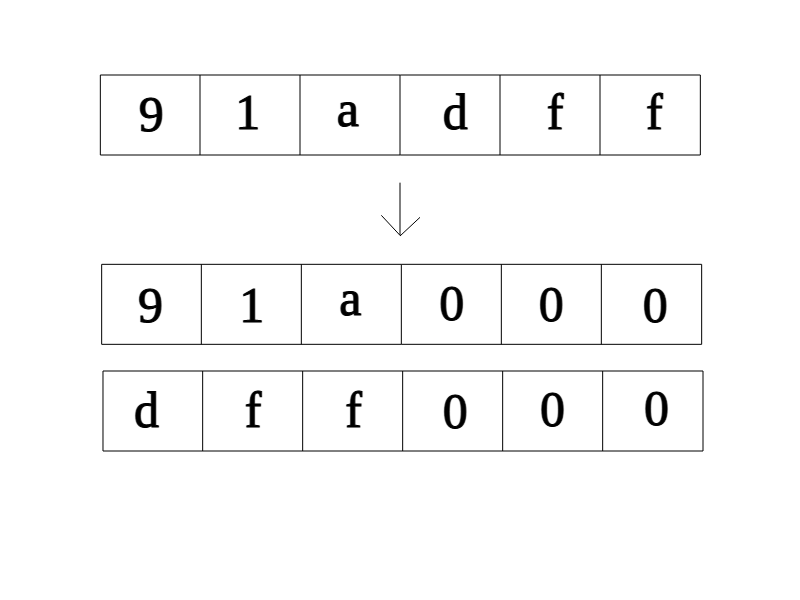
\includegraphics[width=0.9\textwidth]{figures/fundamentals_truncation.png}
    \caption[Illustration: Truncation of words]{Example of a longer word being split into two with the lower bits being set to zero}
    \label{fig:truncation}
\end{figure}

\subsubsection{Word Select}

Word select determines the transmission channel, where 0 means the left channel and 1 means the right one.
It can be changed on a trailing or leading edge of the clock signal and the WS line changes one clock period
before the MSB is transmitted.
For the purpose of what I do in this thesis, WS is not relevant and will be tied to ground unless mentioned otherwise.

\subsection{Pulse Density Modulation}

Pulse Density Modulation (PDM) is one way to represent an analog signal with a binary signal.
The density of high/low signals at a given sampling rate encodes the state of the analog signal.
So the analog signal is encoded using only 1 bit at a high sampling rate.\\
Therefore, a constant bit stream of 1s would represent that the amplitude of the analog signal is maxed out,
while a constant bit stream of 0s would represent that the amplitude of the analog signal is at its lowest value.
Alternating 1s and 0s represent an amplitude of exactly 0.\\\\
While many digital audio systems use Pulse Code Modulation (PCM),
PDM is often used in mobile phones \cite{pdm_utexas} due to its simplicity and low cost. Unlike PDM, PCM uses multiple bits to represent a signal.
PDM is similar to '1-bit-PCM', however, a one-bit wide PCM encoded signal would be much too noisy to be of use.
So to counteract the noise increase of only using 1 bit the signal is 'over sampled', thereby increasing the bandwidth of the system.
The new spectrum that is created by oversampling the signal has such a high frequency that it is out of the audible range of the human ear.
'Noise Shaping' can then be used to 'push' noise into that new spectrum, thus removing it from the audible signal \cite{pdm_texas}.

\section{Microphones}

This section introduces one PDM and one $I^2S$ (which uses PCM) microphone.
These are the microphones that will be used in this thesis.

\subsection{Adafruit I2S MEMS Microphone}

\subsubsection{Technical Specification}

The $I^2S$ MEMS microphone from Adafruit \cite{i2s_mic} is a digital microphone.
It requires a supply voltage between \SI{1.62}{\volt} and \SI{3.6}{\volt} while drawing a current of \SI{600}{\micro\ampere}.
During sleep mode the current draw is reduced to \SI{10}{\micro\ampere}, and the clock frequency is lowered from anything between
\SI{2048}{\kilo\hertz} and \SI{4096}{\kilo\hertz} to \SI{900}{\kilo\hertz}.
A logical high is read for any voltage between 65\% of the supply voltage ($V_{DD}$) and $V_{DD}$ + \SI{0.3}{\volt},
and a logical low is read for any voltage between \SI{-0.3}{\volt} and 35\% of $V_{DD}$ \cite{i2s_mic_datasheet}.

\subsubsection{Pinout}

The breakout board has 6 pins, $V_{DD}$, and Ground (GND), which are responsible for power, as well as 4 data pins.
The output of the microphone can be read on 'Data Out' (DOUT), and the channel (right/left mono audio) can be changed by
changing the voltage of the 'Select' (SEL) pin, which is set to low (left) by default.
The 'bit clock' (BCLK) is the main clock of the device that determines when data is transmitted, and the 'left/right clock' (LRCLK)
controls whether data is transmitted on the left or right channel.
The LRCLK will also be referred to as 'Word Select' (WS) in some instances \cite{i2s_mic_pinout}.

\subsubsection{Timing}

Figure~\ref{fig:i2s_timing} shows the timing diagram of the $I^2S$ microphone.
A clock period should take between \SI{244.14}{\nano\second} and \SI{488.28}{\nano\second}.
A high or low pulse on the clock should be 35\% of the duration of a period.
The maximum delay of the data from a rising edge of the clock should be \SI{65.92}{\nano\second}
and the clock should take no longer than \SI{3.75}{\nano\second} to rise from low to high \cite{i2s_mic_datasheet}.
\\
WS has to change on a falling edge of the clock (BCLK in this case).
Data is sent with the MSB first and delayed by one clock cycle after a change in WS.

\begin{figure}[htb]
    \centering
    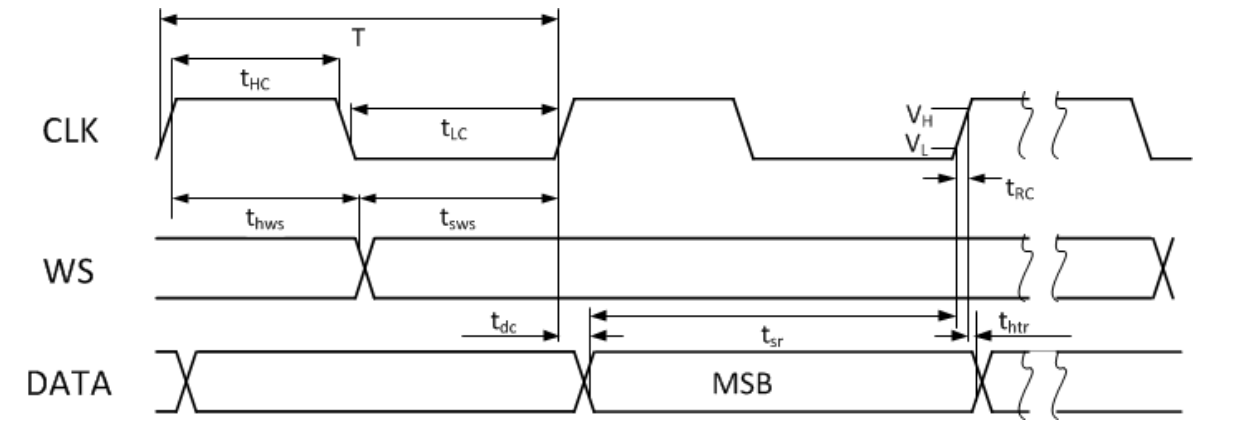
\includegraphics[width=0.9\textwidth]{figures/i2s_timing.png}
    \caption[Timing diagram of the SPH0645LM4H-B $I^2S$ mic \cite{i2s_mic_datasheet}]{Timing diagram of the $I^2S$ microphone}
    \label{fig:i2s_timing}
\end{figure}

\subsection{Adafruit PDM MEMS Microphone}

\subsubsection{Technical Specification}

The PDM MEMS microphone from Adafruit \cite{pdm_mic} is a digital microphone.
It uses the $I^2S$ bus to communicate, but instead of the typical 24-bit encoding of $I^2S$ microphones, PDM microphones only use 1 bit.
It requires a supply voltage between \SI{1.64}{\volt} and \SI{3.6}{\volt} while drawing a current of \SI{600}{\micro\ampere}, with a clock
frequency from \SI{1}{\mega\hertz} to \SI{3.25}{\mega\hertz}.
However, the clock frequency should be reduced to a maximum of \SI{0.23}{\mega\hertz} while the microphone is in 'power-down' mode.
During power down mode, the current draw is reduced to \SI{20}{\micro\ampere}.
A logical high is read for any voltage between 65\% of ($V_{DD}$) and $V_{DD}$ + \SI{0.3}{\volt},
and a logical low is read for any voltage between \SI{-0.3}{\volt} and 35\% of $V_{DD}$ \cite{pdm_mic_datasheet}.

\subsubsection{Pinout}

The breakout board of the PDM microphone, in contrast to the breakout board of the $I^2S$ microphone, only has 5 pins.
$V_{DD}$ and Ground (GND), serve the same purpose, but it only needs 3 data pins.
The output of the PDM microphone can be read on 'PDM Data Out' (DAT), and the PDM microphone also has a SEL pin (also referred to as L/R in the timing diagram),
which works the same way as it does in the $I^2S$ microphone.
However, it only has one clock line (CLK), and no WS \cite{pdm_mic_pinout}.

\subsubsection{Timing}

Figure~\ref{fig:pdm_timing} shows the timing diagram for the PDM microphone.
Based on the clock frequency, a period in normal mode should take between \SI{308}{\nano\second} and \SI{1000}{\nano\second}.
The right channel (PDM R) is latched onto the rising edge of the clock and is enabled if the L/R pin is set accordingly.
It is disabled on the falling edge of the clock.
The left channel (PDM L) is latched onto and thus enabled on a falling edge of the clock (assuming L/R is set accordingly),
and disabled on a rising edge.
According to data acquired from design simulations by the manufacturer,
PDM L and PDM R take at least \SI{18}{\nano\second} while disabling PDM L and PDM R takes at most \SI{16}{\nano\second}.


\begin{figure}[htb]
    \centering
    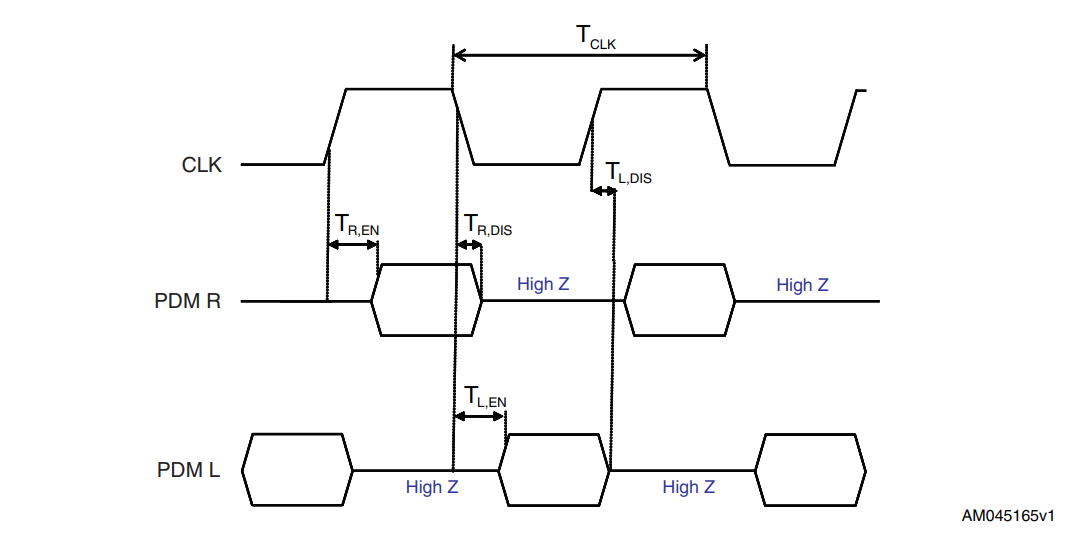
\includegraphics[width=0.9\textwidth]{figures/pdm_timing.png}
    \caption[Timing diagram of the MP34DT01-M PDM MEMS mic \cite{pdm_mic_datasheet}]{Timing diagram of the PDM MEMS microphone}
    \label{fig:pdm_timing}
\end{figure}
